% !TEX TS-program = pdflatex
% !TEX encoding = UTF-8 Unicode

\documentclass{beamer}
 %\documentclass[handout]{beamer}

%\setbeamertemplate{background canvas}[vertical shading][bottom=white,top=structure.fg!25]
% or whatever

\usetheme[compress]{Amsterdam}
%\setbeamertemplate{headline}{}
%\setbeamertemplate{footline}{}
%\setbeamersize{text margin left=0.5cm}
  
\usepackage[english]{babel}
\usepackage{listings}
\usepackage{geometry}
\usepackage{hyperref}
\usepackage{multicol}


\usepackage[utf8]{inputenc}
\usepackage[T1]{fontenc}
\usepackage{lmodern}

\lstset{
basicstyle=\scriptsize\ttfamily,
columns=flexible,
breaklines=true,
numbers=left,
numberstyle=\tiny,
backgroundcolor=\color[rgb]{0.85,0.90,1}
}


\begin{document}
	

\title[Big Data  and Automated Content Analysis]{\textbf{Big Data  and Automated Content Analysis I+II} \\ Week 6 -- Wednesday\\ »Web scraping«}
\author[Anne Kroon]{Anne Kroon \\ ~ \\ \footnotesize{a.c.kroon@uva.nl \\@annekroon} \\ }
\date{11 March 2020}
\institute[UvA]{Afdeling Communicatiewetenschap \\Universiteit van Amsterdam}

%\maketitle
\begin{frame}{}
\titlepage
\end{frame}

\begin{frame}{Today}
\tableofcontents
\end{frame}

%{\setbeamercolor{background canvas}{bg=black}
%\begin{frame}[plain]
%\makebox[\linewidth]{
%\includegraphics[width=\paperwidth,height=\paperheight,keepaspectratio]{process-heel.png}}
%\end{frame}
%}

\section{A first intro to parsing webpages}

\begin{frame}
Let's have a look of a webpage with comments and try to understand the underlying structure.
\end{frame}


{\setbeamercolor{background canvas}{bg=black}
\begin{frame}[plain]
\makebox[\linewidth]{
\includegraphics[width=\paperwidth,height=\paperheight,keepaspectratio]{../../pictures/geenstijl.png}}
\end{frame}
\begin{frame}[plain]
\makebox[\linewidth]{
\includegraphics[width=\paperwidth,height=\paperheight,keepaspectratio]{../../pictures/geenstijl_detail.png}}
\end{frame}

\begin{frame}[plain]
\makebox[\linewidth]{
\includegraphics[width=1.3\paperwidth,height=\paperheight,keepaspectratio]{../../pictures/geenstijl2018-2.png}}
\end{frame}
}


\begin{frame}{Let's make a plan!}
\begin{block}{Which elements from the page do we need?}
\begin{itemize}
\item What do they mean?
\item How are they represented in the source code?
\end{itemize}
\end{block}
\begin{block}{How should our output look like?}
\begin{itemize}
\item What \emph{lists} do we want?
\item \ldots
\end{itemize}
\end{block}
And how can we achieve this?
\end{frame}


\begin{frame}{}
\begin{block}{A first plan}
\begin{enumerate}
\item<2-> Download the page
   \begin{itemize}
   \item<3-> Possibly taking measures to deal with cookie walls, being blocked, etc.
   \end{itemize}
\item<4-> Remove all line breaks (\textbackslash n, but maybe also \textbackslash n\textbackslash r or \textbackslash r) and TABs (\textbackslash t): We want one long string
\item<5-> Try to isolate the comments
   \begin{itemize}
   	\item<5-> Do we see any pattern in the source code? $\Rightarrow$ \emph{last week: if we can see a pattern, we can describe it with a regular expression}
   \end{itemize}
\end{enumerate}
\end{block}

\end{frame}

\begin{frame}[fragile,plain]
\begin{lstlisting}
import requests
import re

URL = 'http://www.geenstijl.nl/mt/archieven/2014/05/das_toch_niet_normaal.html'

# ugly workaround to circumvent cookie wall, not of interest for today
client = requests.session()
r = client.get(URL)
cookies = client.cookies.items()
cookies.append(('cpc','10'))
response = client.get(URL,cookies=dict(cookies))
# end workaround

tekst=response.text.replace("\n"," ").replace("\t"," ")

comments=re.findall(r'<div class="cmt-content">(.*?)</div>',tekst)
print("There are",len(comments),"comments")
print("These are the first two:")
print(comments[:2])
\end{lstlisting}
\end{frame}



\begin{frame}{Some remarks}
\begin{block}{The regexp}<1->
\begin{itemize}
\item {\tt{.*?}} instead of {\tt{.*}} means \emph{lazy} matching. As  {\tt{.*}} matches everything, the part where the regexp should stop would not be analyzed (\emph{greedy} matching) -- we would get the whole rest of the document (or the line, but we removed all line breaks).
\item<2->The parentheses in {\tt{(.*?)}} make sure that the function only returns what's between them and not the surrounding stuff (like {\tt{<div>}} and {\tt{</div>}})
\end{itemize}
\end{block}
\begin{block}{Optimization}<3->
\begin{itemize}
\item Parse usernames, date, time, \ldots
\item Replace \texttt{<p>} tags
\end{itemize}
\end{block}

\end{frame}



\begin{frame}{Further reading}

\begin{block}{Doing this with other sites?}<1->
\begin{itemize}
\item It's basically puzzling with regular expressions. 
\item Look at the source code of the website to see how well-structured it is.
\end{itemize}
\end{block}

%\begin{block}{More powerful modules and packages}<2->
%\begin{itemize}
%\item BeautifulSoup
%\item Scrapy
%\end{itemize}
%\end{block}
\end{frame}



\section{Scraping}
\begin{frame}
OK, but this surely can be doe more elegantly? Yes!
\end{frame}


\begin{frame}{Scraping}
\begin{block}{Geenstijl-example}
\begin{itemize}
\item<1->Worked well (and we could do it with the knowledge we already had)
\item<2->But we can also use existing parsers (that can interpret the structure of the html page)
\item<3->especially when the structure of the site is more complex 
\end{itemize}
\end{block}
\end{frame}

{\setbeamercolor{background canvas}{bg=black}
	\begin{frame}[plain]
	\makebox[\linewidth]{
		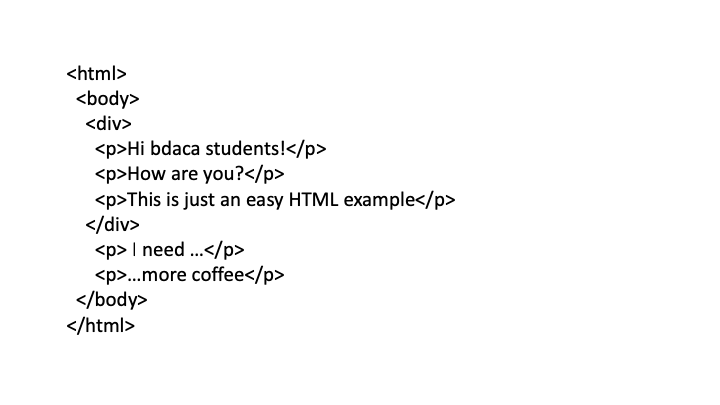
\includegraphics[width=\paperwidth,height=\paperheight,keepaspectratio]{../../pictures/html_example.png}}
\end{frame}
}

{\setbeamercolor{background canvas}{bg=black}
	\begin{frame}[plain]
	\makebox[\linewidth]{
		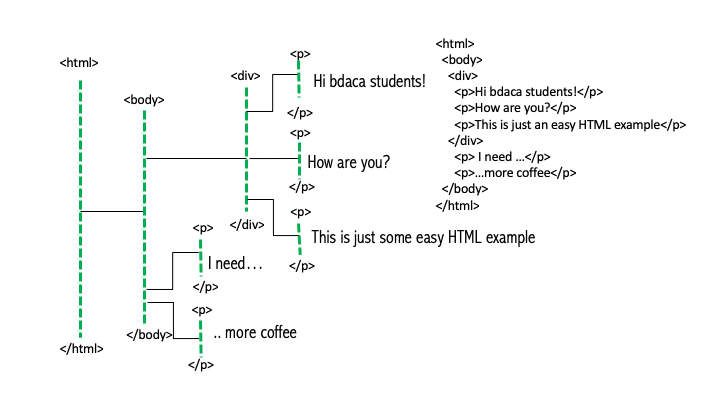
\includegraphics[width=\paperwidth,height=\paperheight,keepaspectratio]{../../pictures/tree_1.png}}
\end{frame}
}

{\setbeamercolor{background canvas}{bg=black}
	\begin{frame}[plain]
	\makebox[\linewidth]{
		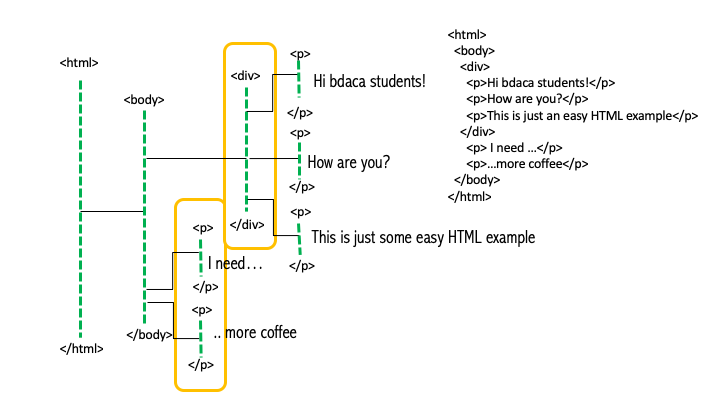
\includegraphics[width=\paperwidth,height=\paperheight,keepaspectratio]{../../pictures/tree_2.png}}
\end{frame}
}

{\setbeamercolor{background canvas}{bg=black}
	\begin{frame}[plain]
	\makebox[\linewidth]{
		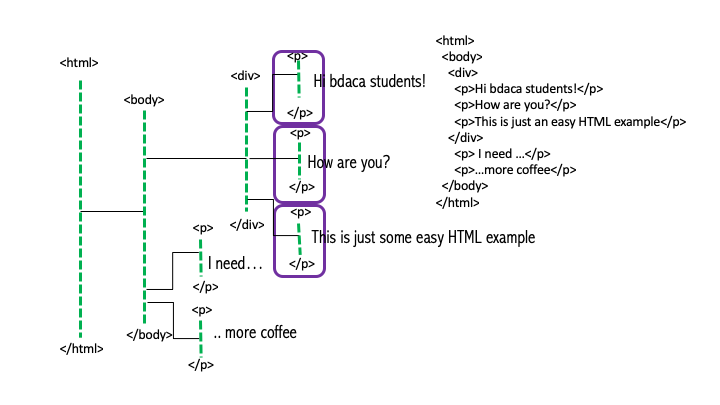
\includegraphics[width=\paperwidth,height=\paperheight,keepaspectratio]{../../pictures/tree_3.png}}
\end{frame}
}

{\setbeamercolor{background canvas}{}
	\begin{frame}[plain]
	\makebox[\linewidth]{
		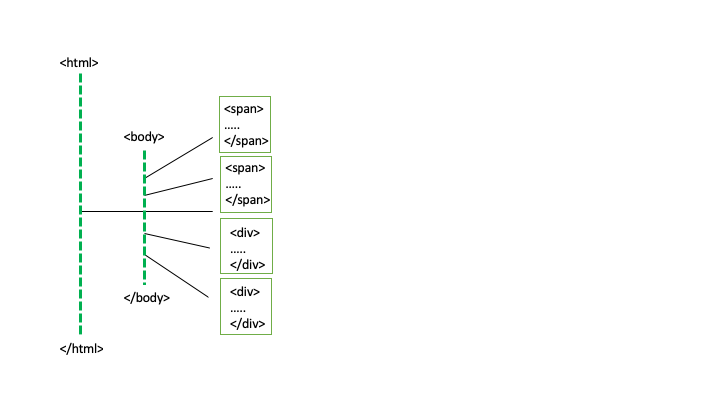
\includegraphics[width=\paperwidth,height=\paperheight,keepaspectratio]{../../pictures/xpath1.png}}
XPATH = ``/html/body/div[1]" refers to which element?
\end{frame}
}

{\setbeamercolor{background canvas}{}
	\begin{frame}[plain]
	\makebox[\linewidth]{
		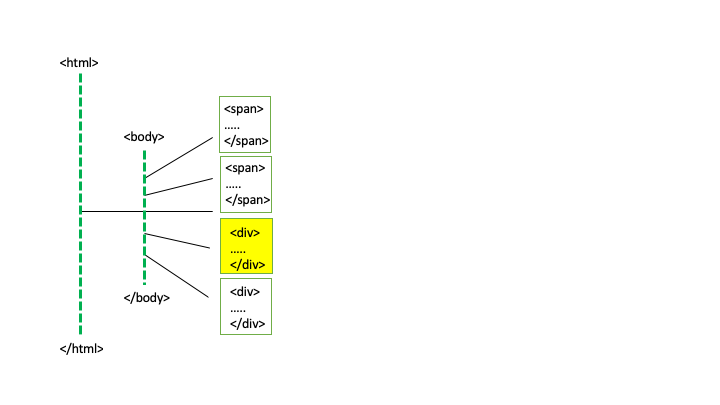
\includegraphics[width=\paperwidth,height=\paperheight,keepaspectratio]{../../pictures/xpath2.png}}
XPATH = ``/html/body/div[1]" refers to which element?
\end{frame}

}


\begin{frame}{What do we need?}
\begin{itemize}
\item <1-> the URL (of course)
\item <2-> the XPATH of the element we want to scrape (you'll see in a minute what this is)
\end{itemize}
\footnotesize{
	\onslide<3->{The following example is based on \url{https://www.kieskeurig.nl/smartphone/product/3518001-samsung-galaxy-a5-2017-goud/reviews}.  It uses the module {\tt{lxml}} }}
\end{frame}


{\setbeamercolor{background canvas}{bg=black}
\begin{frame}[plain]
\makebox[\linewidth]{
\includegraphics[width=\paperwidth,height=\paperheight,keepaspectratio]{../../pictures/kieskeurig2018.png}}
\end{frame}
\begin{frame}[plain]
\makebox[\linewidth]{
\includegraphics[width=\paperwidth,height=\paperheight,keepaspectratio]{../../pictures/kieskeuriginspect2018-1.png}}
\end{frame}
\begin{frame}[plain]
	\makebox[\linewidth]{
		\includegraphics[width=\paperwidth,height=\paperheight,keepaspectratio]{../../pictures/kieskeuriginspect2018-2.png}}
\end{frame}
\begin{frame}[plain]
	\makebox[\linewidth]{
		\includegraphics[width=\paperwidth,height=\paperheight,keepaspectratio]{../../pictures/kieskeuriginspect2018-3.png}}
\end{frame}

}




\begin{frame}{But you can also create your XPATH yourself}
There are multiple different XPATHs to address a specific element.

Some things to play around with:
\begin{itemize}
\item<1-> \texttt{//} means `arbitrary depth' (=may be nested in many higher levels)
\item<2->  \texttt{*} means `anything'. (\texttt{p[2]} is the second paragraph, \texttt{p[*]} are all
\item<3-> If you want to refer to a specific attribute of a HTML tag, you can use \texttt{@}. For example, every \texttt{*[@id="reviews-container"]} would grap a tag like \texttt{<div id=reviews-container'' class='''user-content'}
\item<4->  Let the XPATH end with \texttt{/text()} to get all text
\item<5->  Have a look at the source code (via `inspect elements') of the web page to think of other possible XPATHs!
\end{itemize}
\end{frame}



\begin{frame}{Let's test it!}
	\large{\url{https://www.kieskeurig.nl/wasmachine/product/2483630-siemens-wmn16t3471/reviews}}
\end{frame}


\begin{frame}[fragile]{Let's scrape them!}
\begin{lstlisting}
from lxml import html
import requests

response = requests.get('https://www.kieskeurig.nl/wasmachine/product/2483630-siemens-wmn16t3471/reviews')
tree = html.fromstring(response.text)

# we extract all relevant elements using their XPATH
reviews =  tree.xpath('//div[@class="reviews-single__text"]')
# alternatively, we can use their CSS selector:
# reviews =  tree.cssselect("div.reviews-single__text")

# but we don't want the elements, we want their text
review_texts = [e.text_content().strip() for e in reviews]

print (len(reviews),"reviews scraped. Showing the first 60 characters:")
i=0
for review in review_texts:
    print("Review",i,":",review[:60])
    i+=1
\end{lstlisting}
\tiny{If you want to use CSS selectors, you need to \texttt{sudo pip3 install cssselect} first}
\end{frame}



\begin{frame}[fragile]{The output -- perfect!}
\begin{lstlisting}
20 reviews scraped. Showing the first 60 characters:
Review 0 : Siemens WMN16T3471 nu 4 maanden in gebruik in massagesalon. 
Review 1 : Na een eerder positief review kort na aankoop nu een bijgest
Review 2 : Helaas ben ik teleurgesteld in dit product wegens de navolge
Review 3 : Ik ben heel blij met mijn nieuwe wasmachine: 

Wat is hij st
Review 4 : Ik heb de wasmachine nu net een paar dagen in huis en heb al
Review 5 : Na 25 jaar hebben we afscheid moeten nemen van onze degelijk
\end{lstlisting}
\end{frame}

\section{Scaling up}
\begin{frame}[plain]
	Scaling up
\end{frame}


\begin{frame}[fragile]{But this was on \emph{one} page only, right?}
Next step: Repeat for each relevant page.

\begin{block}{Possibility 1: Based on url schemes}
	If the url of one review page is \url{https://www.hostelworld.com/hosteldetails.php/ClinkNOORD/Amsterdam/93919/reviews?page=2}

\ldots then the next one is probably?
\end{block}

\pause

$\Rightarrow$ you can construct a list of all possible URLs:

\begin{lstlisting}
baseurl = 'https://www.hostelworld.com/hosteldetails.php/ClinkNOORD/Amsterdam/93919/reviews?page='

allurls = [baseurl+str(i+1) for i in range(20)]
\end{lstlisting}	
	
\end{frame}



\begin{frame}[fragile]{But this was on \emph{one} page only, right?}
	Next step: Repeat for each relevant page.
	
	\begin{block}{Possibility 2: Based on XPATHs or CSS Selectors}
	Use XPATH to get the url of the next page (i.e., to get the link that you would click to get the next review)
	\end{block}
	
\end{frame}


\begin{frame}{Recap}
\begin{block}{General idea}
\begin{enumerate}
\item Identify each element by its XPATH or CSS Selector (look it up in your browser) 
\item Read the webpage into a (loooooong) string
\item Use the XPATH  or CSS Selectors to extract the relevant text into a list (with a module like lxml)
\item Do something with the list (preprocess, analyze, save)
\item Repeat
\end{enumerate}
\footnotesize{Alternatives: scrapy, beautifulsoup, regular expressions, \ldots}
\end{block}
\end{frame}


\begin{frame}{Last remarks}
	\begin{block}{There is often more than one way to specify an XPATH}
		\begin{enumerate}
			%\item You can usually leave away the namespace (the \texttt{x:})
			\item Sometimes, you might want to use a different suggestion to be able to generalize better (e.g., using the \emph{attributes} rather than the \emph{tags})
			\item in that case, it makes sense to look deeper into the structure of the HTML code, for example with ``Inspect Element'' and use that information to play around with different possibilities
		\end{enumerate}
	\end{block}
\end{frame}


{\setbeamercolor{background canvas}{bg=black}
	\begin{frame}[plain]
		\makebox[\linewidth]{
			\includegraphics[width=1.5\paperwidth,height=\paperheight,keepaspectratio]{../../pictures/kieskeuriginspect2018-2.png}}
	\end{frame}
}

\section{Next steps}
\begin{frame}
Next steps
\end{frame}

%
%
%\begin{frame}{From now on\ldots}
%\ldots focus on individual projects!
%\makebox[\linewidth]{
%\includegraphics[width=\paperwidth,height=.6\paperheight,keepaspectratio]{../../pictures/projectlastminute}}
%\end{frame}


\begin{frame}{Friday}


\begin{itemize}
\item Write a scraper for a website of your choice!
\item Choose an easy site where you do not have to log on and where there is no dynamically generated content (if you need that, look at the Appendix on Selenium)
\end{itemize}

\pause

Scraping can be difficult, but it is also one of the most important data collection methods. Chances are very high you'll need it as a part of your final project. Try writing a scraper, and ask questions next week.

\end{frame}


\begin{frame}[plain]{}
	\makebox[\linewidth]{
		\includegraphics[width=1.2\paperwidth,height=\paperheight,keepaspectratio]{../../pictures/iens.png}}
\end{frame}




\end{document}


